%*********************************************
\section{Markov Chain}\label{app:markov_chain}
%*********************************************

%---------------0---------------------------------
\subsection{Discrete-State}\label{app:mc_discrete}
%-------------------------------------------------

% Markov Chain
Markov chain on a discrete-state space $\mathcal{S}$ is defined as a sequence of random variables $\{\mathcal{X}^{(i)}, i \geq 0\}$ where the indices represents successive time, step, or iteration,
\emph{such that the conditional probability distribution of $\mathcal{X}^{(i+1)}$ follows the Markov assumption}.
\marginpar{Markov chain}
That is,
\begin{equation}
  \mathcal{X}^{(i+1)} | \mathcal{X}^{(i)}, \mathcal{X}^{(i-1)}, \ldots, \mathcal{X}^{(0)} = \mathcal{X}^{(i+1)} | \mathcal{X}^{(i)}
\label{eq:markov_property}
\end{equation}
Put differently, the future value depends on the past only through the present value \cite{Geyer2011} and Sokal.

% Ingredients
A discrete-state Markov chain is fully defined by its joint probability (cite Sokal).
\begin{equation}
	\begin{split}
  \mathbb{P}(\mathcal{X}^{(i+1)} & = x^{(i+1)}, \mathcal{X}^{(i)} = x^{(i)}, \ldots, \mathcal{X}^{(0)} = x^{(0)}) = \\
	& \mathbb{P}(\mathcal{X}^{(0)} = x^{(0)}) \cdot \mathbb{P}(\mathcal{X}^{(1)} = x^{(i+1)} | \mathcal{X}^{(0)} = x^{(i+1)}) \cdot \ldots \\
	& \cdot \mathbb{P}(\mathcal{X}^{(i+1)} | \mathcal{X}^{(i)}) \cdot
	\end{split}
\label{eq:markov_chain_joint_probability}
\end{equation}
The specification consists of three main components:
\begin{itemize}

	\item The state space $\mathcal{S}$, all the possible outcomes of the random variables $\{\mathcal{X}^{(i)}\}$.
	\marginpar{Discrete state space}
	The state space considered here is discrete with $D$ elements, $\mathcal{S} = \{x_1, x_2, \ldots, x_D \}$.
	
	\item The initial probability distribution $\pi^{(0)}$.
	\marginpar{Initial distribution}
	This is the (marginal) probability distribution of $\mathcal{X}^{(0)}$ (or the marginal distribution of the chain at $i = 0$). That is,
	\begin{equation}
		\mathbb{P}(\mathcal{X}^{(0)} = x_d) = \pi^{(0)}_d \,\,\, \forall d
	\label{eq:markov_chain_initial_distribution}
	\end{equation}
	
	\item The \emph{transition probability matrix} $P$, an $D \times D$ with elements $p_{x,y} \geq 0.0$ and $\sum_y p_{x,y} = 1.0$.
	\marginpar{Transition probability}
	Each element is the conditional probability between two states. That is,
	\begin{equation}
		p_{x,y} = \mathbb{P}(\mathcal{X}^{(i+1)} = y | \mathcal{X}^{(i)} = x) \,\,\, \forall x,y \in \mathcal{S}
	\label{eq:markov_chain_transition_matrix_element}
	\end{equation}
	Transition probability matrix is said to be \emph{stationary} if it does not depend on a particular step $i$.
	\marginpar{Stationary transition probability}
	For all practical purposes, most \gls[hyper=false]{mcmc} algorithms rely on a stationary transition probability \cite{Geyer2011}.
\end{itemize}

% Example of Chain
As an example of a discrete-state Markov chain, consider a $3$-state Markov chain representing changes of human health condition with $\mathcal{S} = \{\text{Healthy}, \text{Sick}, \text{Dead}\}$ and a transition probability matrix $P$,
\begin{equation}
  P =  
    \begin{pmatrix}
      \mathbb{P}(H | H)  & \mathbb{P}(S | H) & \mathbb{P}(D | H)\\
      \mathbb{P}(H | S)  & \mathbb{P}(S | S) & \mathbb{P}(D | S)\\
      \mathbb{P}(H | D)  & \mathbb{P}(S | D) & \mathbb{P}(D | D)\\
    \end{pmatrix} =
		\begin{pmatrix}
		  0.75  & 0.20 & 0.05\\
      0.65  & 0.15 & 0.20\\
      0.00  & 0.00 & 1.00\\
		\end{pmatrix}
\label{eq:app_transition_probability_matrix}
\end{equation}
The Markov chain is graphically represented in Fig.~\ref{fig:app_markov_chain}.
\begin{figure}[bth]
	\centering
	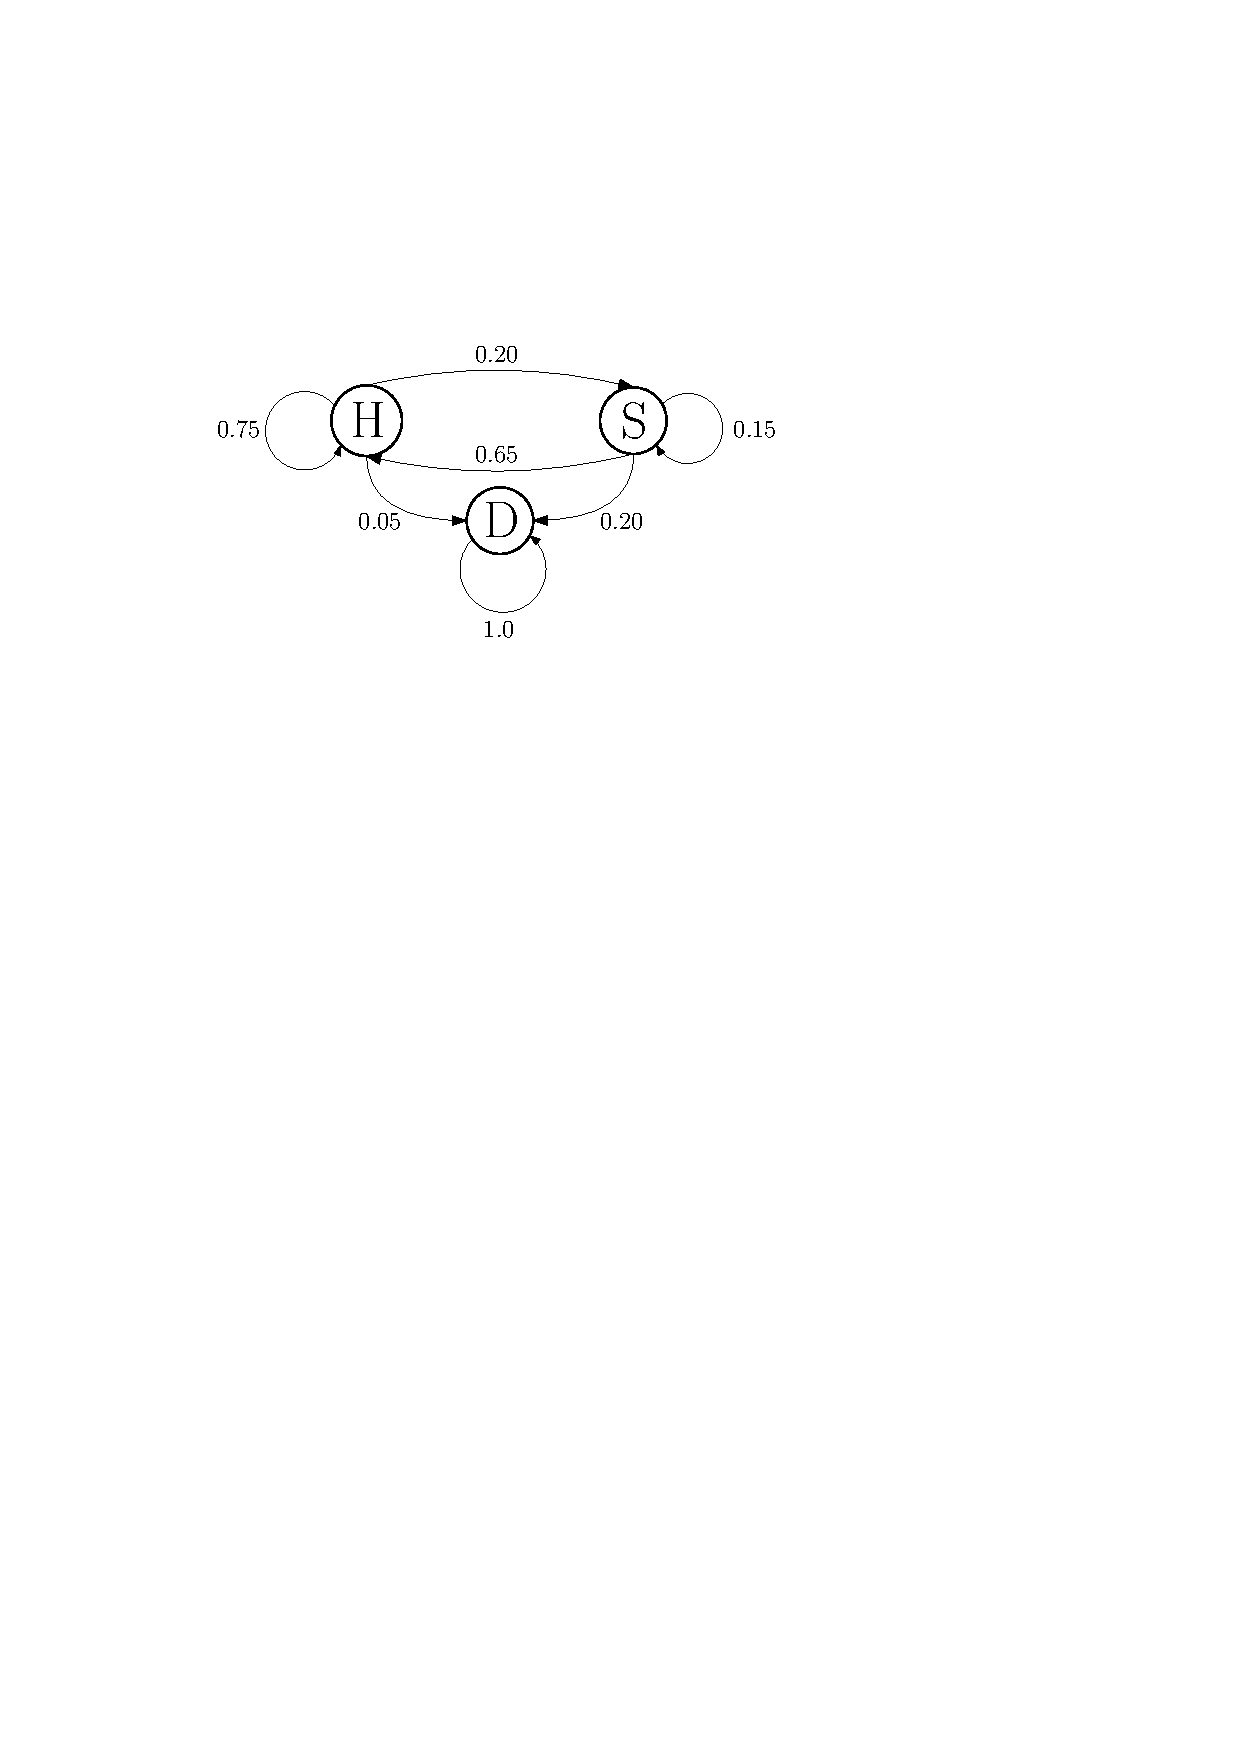
\includegraphics[width=1.0\textwidth]{../figures/chapter5/figures/markov_chain.pdf}
	\caption[Illustration of a $3$-State Markov Chain]{An illustration of a $3$-State Markov chain with the transition probability given by the matrix $P$ in Eq.~(\ref{eq:app_transition_probability_matrix}).}
	\label{fig:app_markov_chain}
\end{figure}

% Irreducible Chain
\begin{figure}[bth]
	\centering
	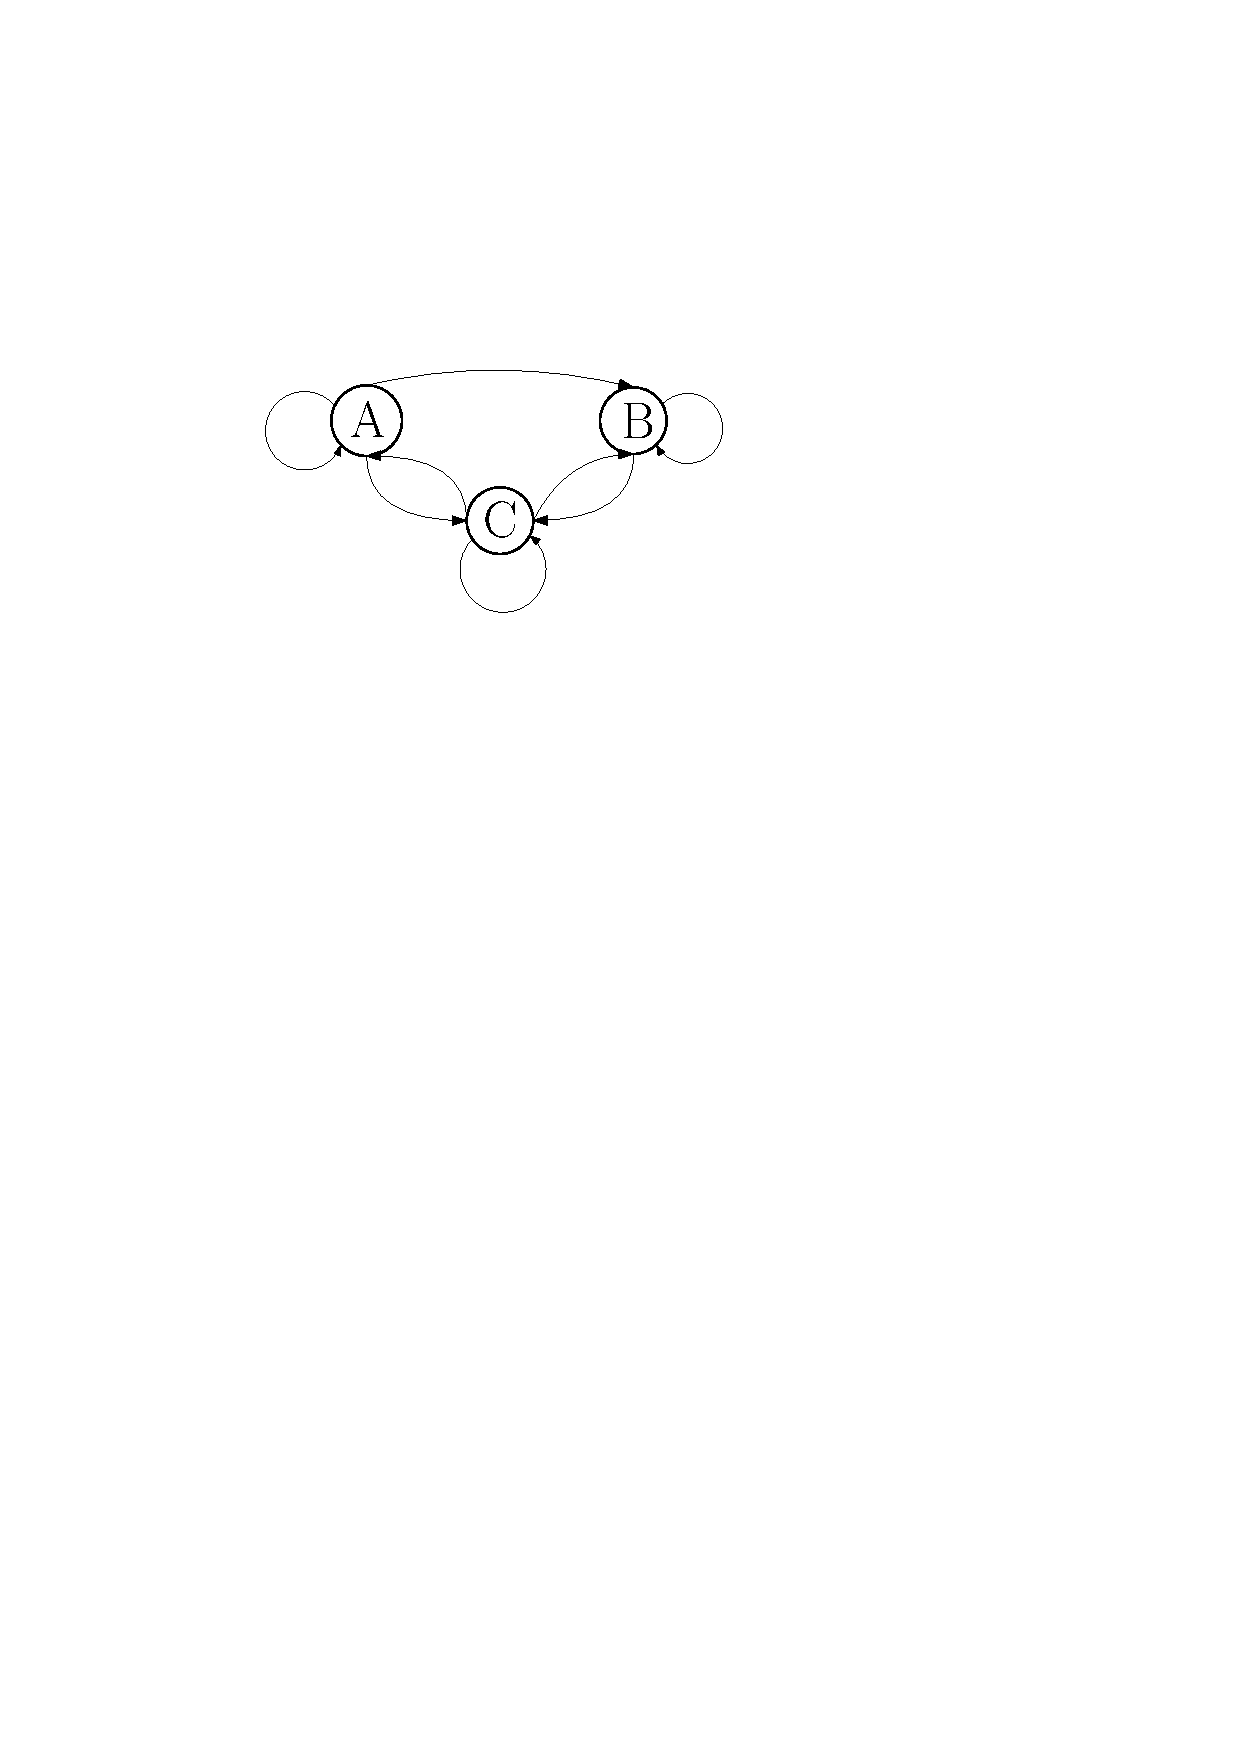
\includegraphics[width=1.0\textwidth]{../figures/chapter5/figures/markov_chain_irreducible.pdf}
	\caption[Illustration of an irreducible $3$-State Markov Chain]{An illustration of an irreducible $3$-State Markov chain.}
	\label{fig:app_markov_chain_irreducible}
\end{figure}

% Period of a Chain and Aperiodicity
\normdoublefigure[pos=tbhp,
                  mainlabel={fig:app_markov_chain_periodicity},
                  maincaption={Examples of periodic and aperiodic chains. (Left) an example of a periodic $3$-state Markov chain. In this case, all states have the the same period of $3$ steps. (Right) an example of aperiodic $3$-state Markov chain, that is all states are aperiodic.},%
									mainshortcaption={Examples of periodic and aperiodic chains.},
                  leftopt={width=0.45\textwidth},
                  leftlabel={fig:app_markov_chain_periodic},
                  leftcaption={Periodic chain},
                  %leftshortcaption={},%
                  rightopt={width=0.45\textwidth},
                  rightlabel={fig:app_markov_chain_aperiodic},
                  rightcaption={Aperiodic chain},
                  %rightshortcaption={},
                  %spacing={\hfill}
                 ]
{../figures/chapter5/figures/markov_chain_periodic}
{../figures/chapter5/figures/markov_chain_aperiodic}

% Stationary Distribution

% Markov Chain Convergence

% Ergodic Theorem

%-----------------------------------------------------
\subsection{Continuous-State}\label{app:mc_continuous}
%-----------------------------------------------------

% Markov Chain

% Ingredients

% Transition Kernel

% Ergodic Theorem

% Some difficulty

